% Compile with:
% latexmk -pdf -pvc -interaction=nonstopmode
%\documentclass[aspectratio=169,10pt,draft]{beamer}
\documentclass[aspectratio=169, 10pt]{beamer}
\usetheme{UniBern}
\title{Adaptation Mechanisms Of Zebrafish Respiratory Organ To Endurance Training}
\author{David Haberthür \and
	Dea Aaldijk \and
	Matthias Messerli \and
	Fluri A.\ M.\ Wieland \and
	Oleksiy Khoma \and
	Helena Röss \and
	Ruslan Hlushchuk}
\institute{Institute of Anatomy\\University of Bern\\Switzerland}
\date{June 5, 2019 | \href{https://www.bruker.com/events/micro-ct-users-meeting.html}{Bruker micro-CT Users Meeting 2019}}

\includeonlyframes{current}
%then....
%\begin{frame}[label=current]
%\end{frame}

\usepackage[english]{babel}
\usepackage{microtype}
\usepackage[backend=biber,
	style=numeric,
	url=false,
	isbn=true,
	maxbibnames=1,
	sorting=none,
	backref=true]{biblatex}
	\addbibresource{../../Documents/library.bib}
\usepackage{graphicx}
\usepackage{tikz}
\usepackage[detect-all=true, range-phrase=--, range-units=single, binary-units=true]{siunitx}
\usepackage[absolute,overlay]{textpos} %for the \source{} command
\usepackage{gitinfo2}
\usepackage[version=4]{mhchem}
\usepackage{xspace}
\usepackage{ccicons}
\usepackage{multimedia}
\usepackage{animate}

\usepackage{pgfplots}
\pgfplotsset{compat=newest}
\usepackage[eulergreek]{sansmath}
\pgfplotsset{
  tick label style = {font=\sansmath\sffamily},
  every axis label = {font=\sansmath\sffamily},
  legend style = {font=\sansmath\sffamily},
  label style = {font=\sansmath\sffamily}
}

% Some often used abbreviations
\newcommand{\imsize}{\linewidth} % set global image width
\newcommand{\everyframe}{1} % use only every nth frame for the movies
\newlength\imagewidth % needed for scalebars
\newlength\imagescale % needed for scalebars
\newcommand{\uct}{\si{\micro}CT\xspace} % make our life easier

% Easily fill a frame with the whole image.
% Based on http://tex.stackexchange.com/a/334758/828,
\newcommand{\fullframeimage}[1]{%
	\begin{tikzpicture}[remember picture,overlay]%
		\node[xshift=0,yshift=0] at (current page.center){%
			\includegraphics[width=\paperwidth]{#1}};%		
	\end{tikzpicture}%
}

% Acknowledge images just below them
% Based on https://tex.stackexchange.com/a/206925/828
%\newcommand{\source}[2]{\par\hfill\tiny \href{http://#1}{#1} #2}
% Based on https://tex.stackexchange.com/a/282637
\newcommand{\source}[2]{%
	\raisebox{-1ex}{\makebox[0pt][r]{\tiny \href{http://#1}{#1} #2}}
}

% Define us our custom footer
\defbeamertemplate{footline}{unibe}{%
	\hspace*{0.6cm}%
	v. \href{https://github.com/habi/20190605_BrukerUserMeeting/commit/\gitHash}{\gitAbbrevHash}%
	\hspace*{\fill}%
	\insertframenumber\,/\,\inserttotalframenumber%
	\hspace*{1.2cm}%
	\vskip2pt%
}
\setbeamertemplate{footline}[unibe]

% Format bibliography for beamer
% http://tex.stackexchange.com/a/10686/828
\renewbibmacro{in:}{}
% http://tex.stackexchange.com/a/13076/828
\AtEveryBibitem{%
	\clearfield{journaltitle}
	\clearfield{pages}
	\clearfield{volume}
	\clearfield{number}
	\clearfield{editors}
	\clearlist{editors}
	\clearname{editors}
	\clearfield{issn}
}


\begin{document}
% We want no footline on the title page, http://tex.stackexchange.com/a/18829/828 helps
{%
	\setbeamertemplate{footline}{}%
	\begin{frame}%
		\maketitle
	\end{frame}%
}

%\begin{frame}
%	\frametitle{Contents}
%	\tableofcontents
%\end{frame}

\begin{frame}
	\frametitle{Hello!}
	\begin{itemize}
		\item<1-> University of Bern, Switzerland
		\item<1-> Institute of Anatomy
		\item<1-> Group for topographic and clinical Anatomy
		\item<1-> \uct-Team: Ruslan Hlushchuk, David Haberthür, Oleksiy-Zakhar Khoma, Fluri Wieland, Carlos Correa Shokiche
		\item<1-> Biomedical research
		\begin{itemize}
			\item microangioCT~\cite{Hlushchuk2018}: Tumor vasculature, angiogenesis in the heart, musculature
			\item Cancer research: Melanoma
			\item Lung imaging: Tumor detection and classification
			\item Physiology: Zebrafish musculature and gills
		\end{itemize}
		\item<1-> SkyScan 1172 \& 1272 \visible<2->{\& 2214}
	\end{itemize}
\end{frame}

\begin{frame}
	\frametitle{Why?}
	\begin{itemize}
		\item Adaptation of respiratory organ to endurance training
		\item Study \ce{O2} metabolism
	\end{itemize}
\end{frame}

\begin{frame}
	\frametitle{Oxygen pathway}
	\begin{columns}
		\begin{column}{0.618\linewidth}
			\begin{itemize}
				\item<1-> Insects: Spiracles \& Trachea
				\item<2-> Bony fishes: Gills
				\item<3-> Mammals: Lungs
			\end{itemize}
		\end{column}
		\begin{column}{0.382\linewidth}
			\only<1>{%
				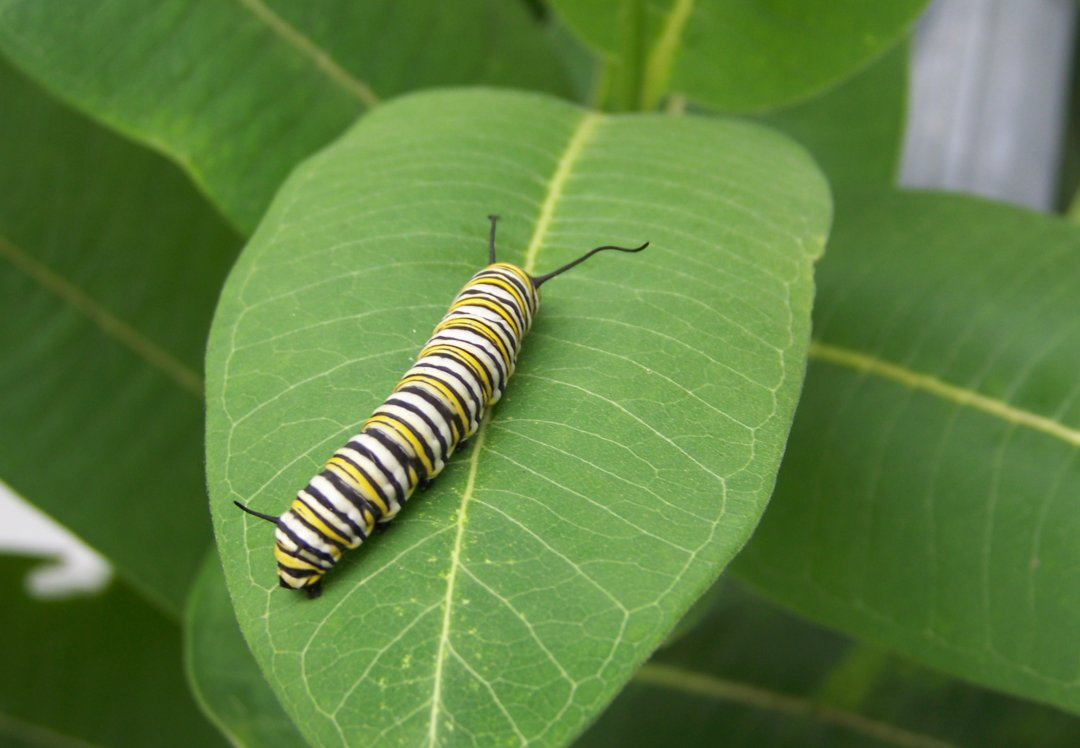
\includegraphics[width=\imsize]{./img/2746294525_52566921c8_o}
				\source{flic.kr/p/5bFtFB}{\ccbyncsa}
				}
			\only<2>{%
				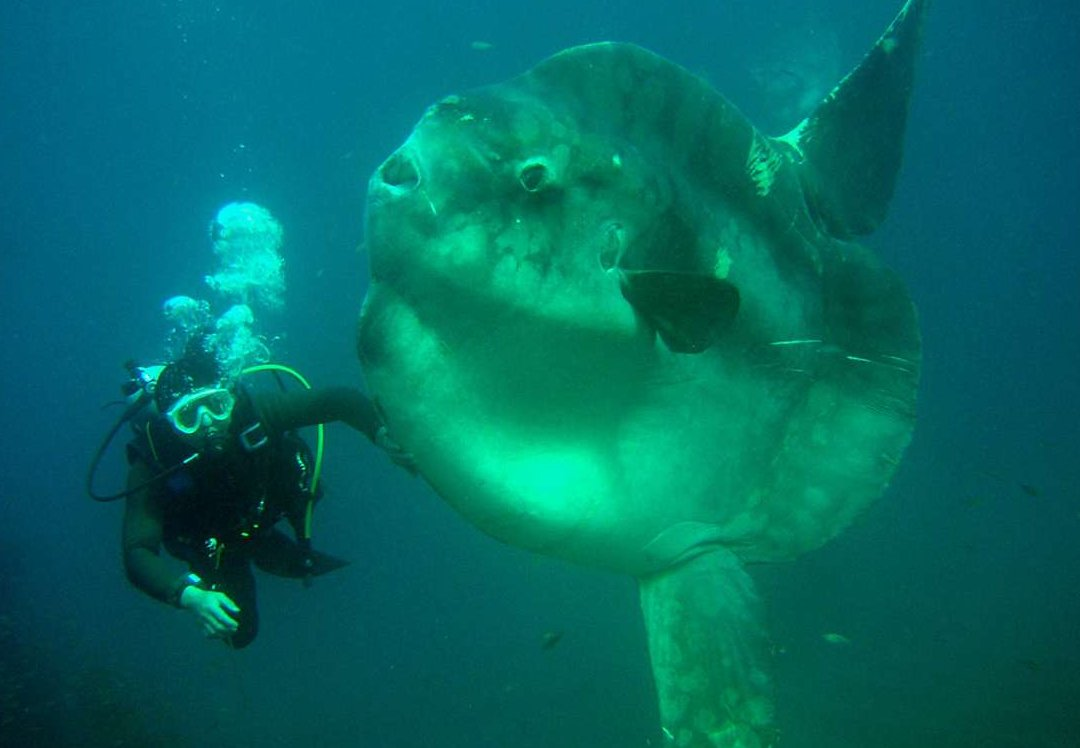
\includegraphics[width=\imsize]{./img/Bump_head_sunfish}%
				\source{enwp.org/molidae}{\ccbysa}
				}
			\only<3>{%
				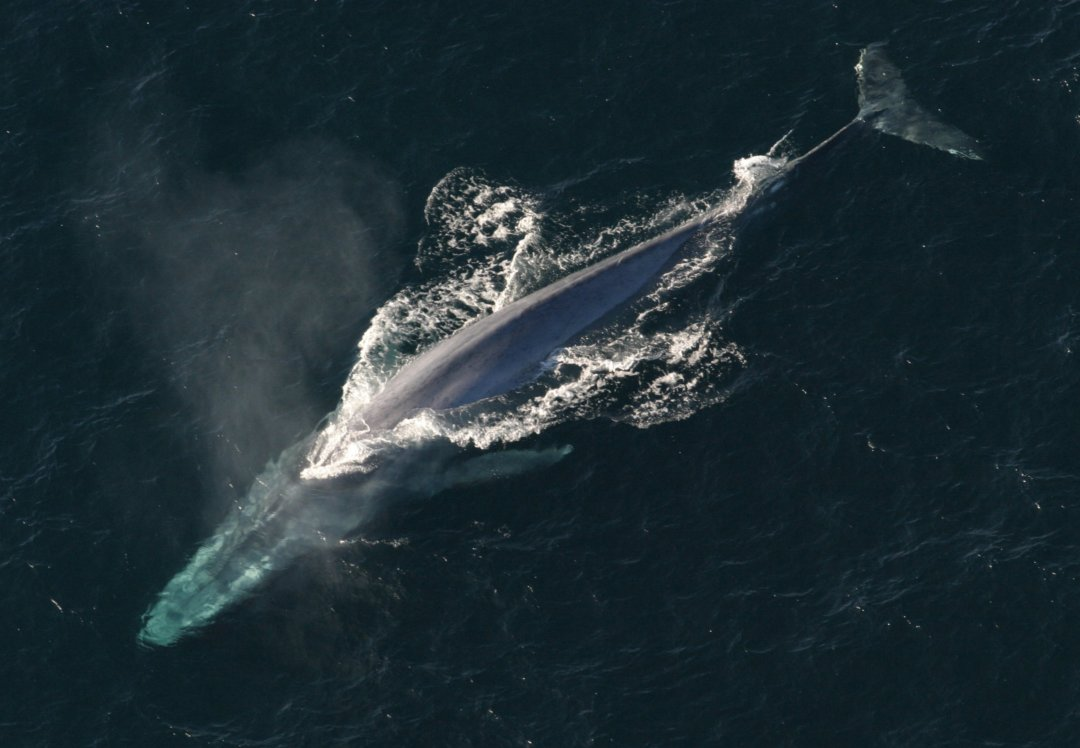
\includegraphics[width=\imsize]{./img/Anim1754_-_Flickr_-_NOAA_Photo_Library}%
				\source{enwp.org/bluewhale}{\ccPublicDomain}
				}
		\end{column}
	\end{columns}
\end{frame}

\begin{frame}
	\frametitle{Biology}
	% Image from https://teacheratsea.files.wordpress.com/2011/07/gills-an-o2.jpg
	\centering
	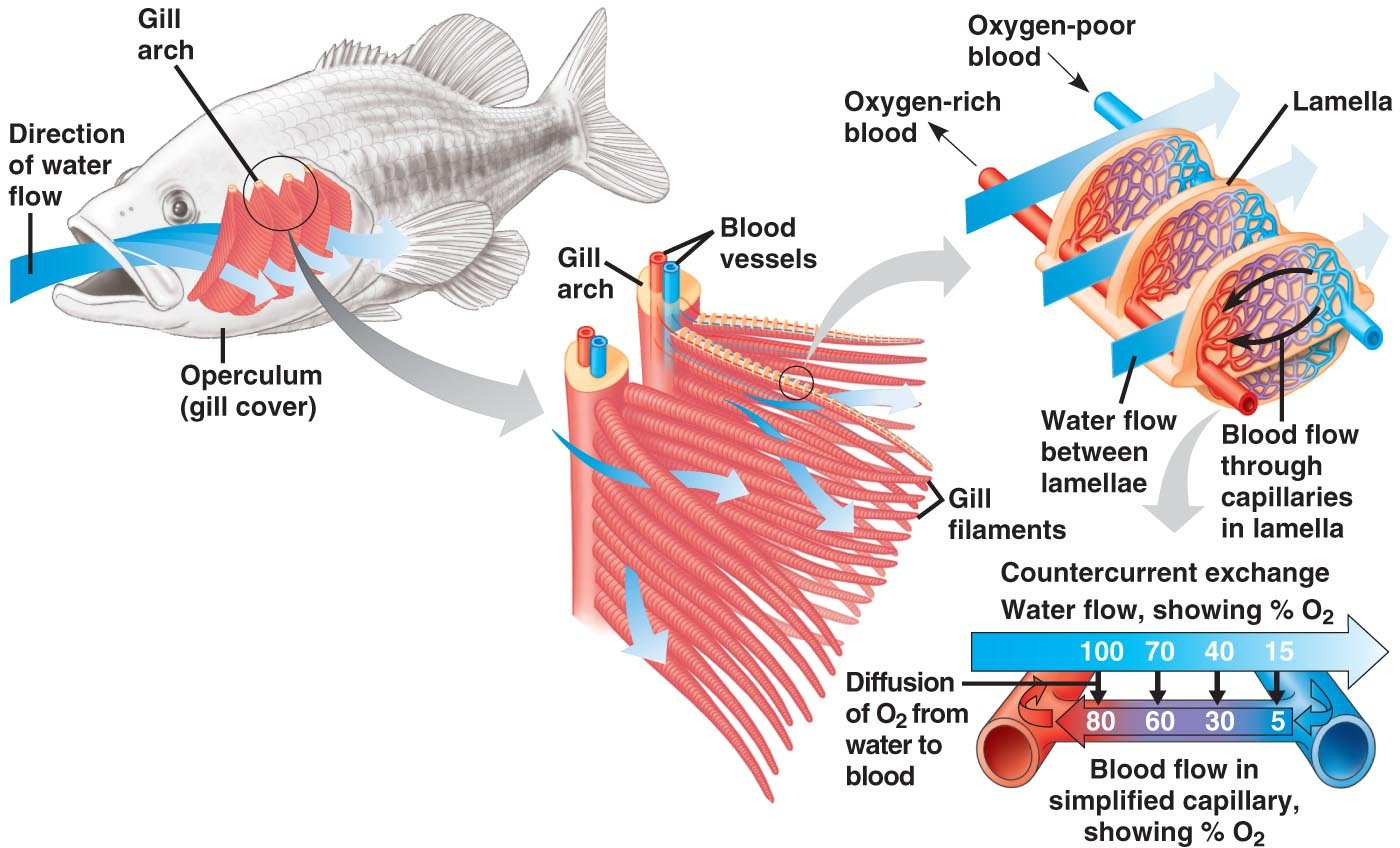
\includegraphics[width=0.618\linewidth]{./img/gills-an-o2}%
	\source{Campbell Biology: Concepts \& Connections}{\cite{Taylor2017}}
\end{frame}

\begin{frame}
	\frametitle{Adaptation to training exercise}
	\begin{itemize}
		\item Increased body length and weight
		\item Skeletal and heart muscle hypertrophy
		\item Induction of angiogenesis in skeletal muscle
		\item Increase in haematocrit
	\end{itemize}
\end{frame}

\begin{frame}
	\frametitle{How?}
		\begin{columns}
	\begin{column}{0.618\linewidth}
		\begin{itemize}
			\item<1-> Fish training according to \textcite{Palstra2010}
			\item<3-> Morphological measurement
			\item<4-> Respirometry
			\item<5-> Electron microscopy
			\item<6-> \uct imaging
			\begin{itemize}
				\item<7-> Delination
				\item<8-> Analysis
			\end{itemize}
		\end{itemize}
	\end{column}
	\begin{column}{0.382\linewidth}
		\only<1>{
			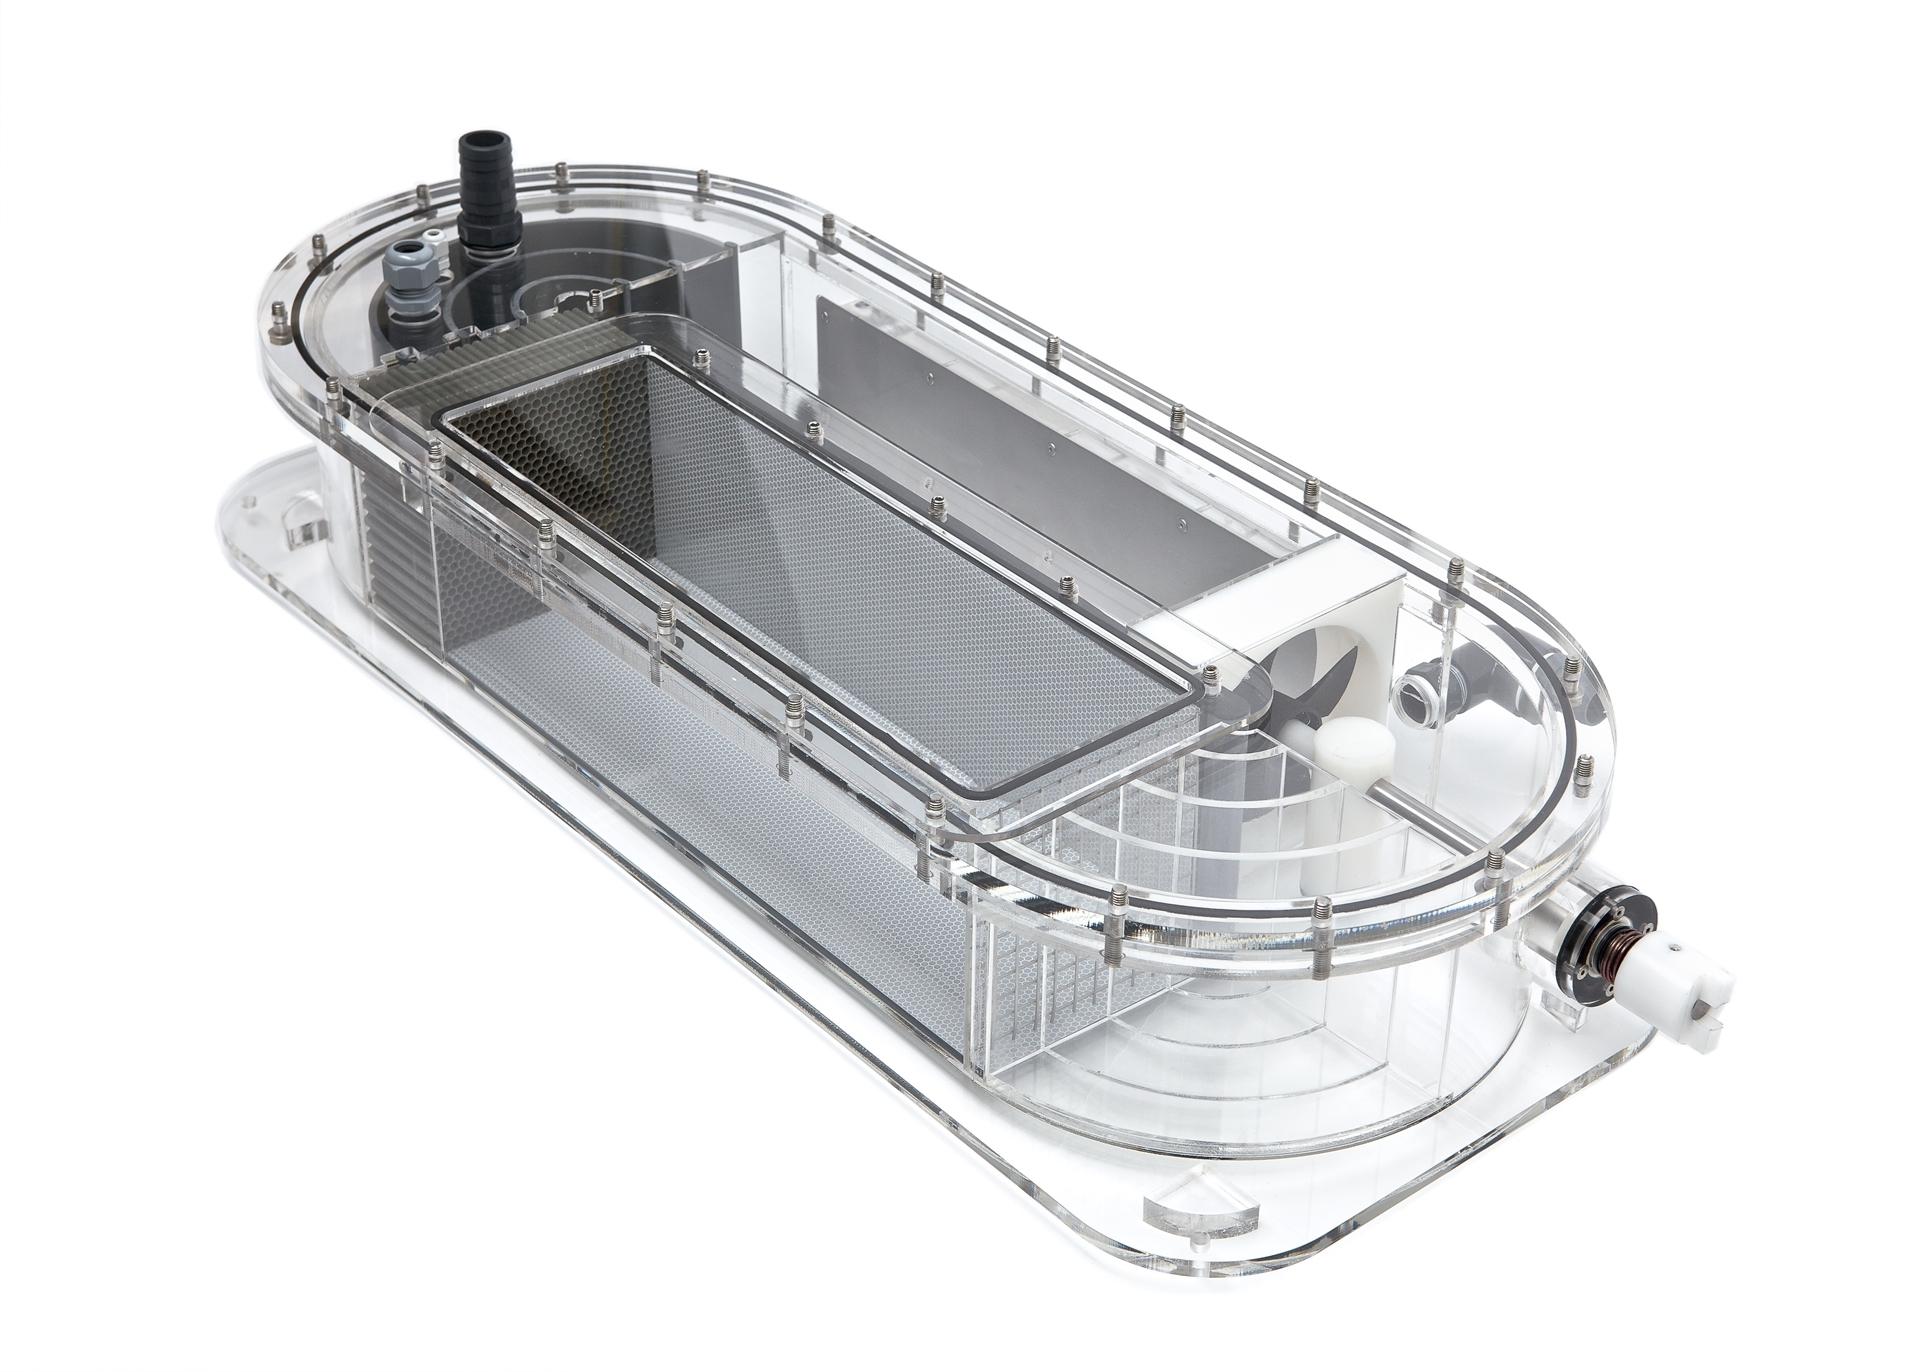
\includegraphics[width=\linewidth]{./img/0001713_swim-tunnel-5-l-230-v-50-hz}%
			\source{loligosystems.com/swim-tunnel-5-l-230-v-50-hz}{}
			}
		\only<2>{
			\animategraphics[loop,autoplay,width=\linewidth]{25}{./mov/fishvideo/fishvideo_}{0001}{0100}
			}
		\only<5>{EM-Bilder}
		\includegraphics<6>[width=\linewidth]{./img/Overviews}%
		\includegraphics<7>[width=\linewidth]{./img/CTAn}%
		\only<8>{
			\animategraphics[loop,autoplay,width=\linewidth]{25}{./mov/coder/coder-}{0}{133}
			}
		\end{column}	
	\end{columns}	
\end{frame}

\begin{frame}
	\frametitle{What?}
	\begin{itemize}
		\item Endurance
		\item Body size
		\item Gill structure
		\item Gill volume
		\item Gill complexity
		\item \ce{O2 consumption}
	\end{itemize}
\end{frame}

\begin{frame}
	\frametitle{Fish morphology}
	\includegraphics<1>[width=\linewidth]{./img/Endurance}
	\includegraphics<2>[width=\linewidth]{./img/Lengths}
	\includegraphics<3>[width=\linewidth]{./img/Weights}
\end{frame}

\begin{frame}
	\frametitle{Fish morphology}
	\only<1>{% This file was created by matplotlib2tikz v0.7.4.
\begin{tikzpicture}

%\definecolor{ubRed}{rgb}{0.83921568627451,0,0.168627450980392}

\begin{axis}[
%axis line style={white!80.0!black},
%legend cell align={left},
%legend style={at={(0.03,0.97)}, anchor=north west, draw=white!80.0!black},
%tick align=outside,
%x grid style={white!80.0!black},
%xmajorticks=false,
xmin=-0.5, xmax=1.5,
%xtick style={color=white!15.0!black},
xtick={0,1},
xticklabels={Before Training,After Training},
%y grid style={white!80.0!black},
ylabel={Water current speed [\si{\centi\metre\per\second}]},
%ymajorgrids,
%ymajorticks=false,
%ymin=0, %ymax=51.4054500165907,
%ytick style={color=white!15.0!black}
]
\path [draw=black, fill=ubGrey]
(axis cs:-0.396,30)
--(axis cs:-0.004,30)
--(axis cs:-0.004,40)
--(axis cs:-0.396,40)
--(axis cs:-0.396,30)
--cycle;
\path [draw=black, fill=ubRed]
(axis cs:0.004,30)
--(axis cs:0.396,30)
--(axis cs:0.396,40)
--(axis cs:0.004,40)
--(axis cs:0.004,30)
--cycle;
\path [draw=black, fill=ubGrey]
(axis cs:0.604,33.75)
--(axis cs:0.996,33.75)
--(axis cs:0.996,40)
--(axis cs:0.604,40)
--(axis cs:0.604,33.75)
--cycle;
\path [draw=black, fill=ubRed]
(axis cs:1.004,40)
--(axis cs:1.396,40)
--(axis cs:1.396,47.5)
--(axis cs:1.004,47.5)
--(axis cs:1.004,40)
--cycle;
\addplot [only marks, draw=black, fill=ubGrey, colormap/blackwhite]
table{%
x                      y
};
%\addlegendentry{Control}
\addplot [only marks, draw=ubRed, fill=ubRed, colormap/blackwhite]
table{%
x                      y
};
%\addlegendentry{Swimmer}
\draw[draw=black,fill=ubGrey,line width=0.45pt] (axis cs:0,0) rectangle (axis cs:0,0);
\addlegendimage{ybar,ybar legend,draw=black,fill=ubGrey,line width=0.45pt};
%\addlegendentry{Control}

\draw[draw=black,fill=ubRed,line width=0.45pt] (axis cs:0,0) rectangle (axis cs:0,0);
\addlegendimage{ybar,ybar legend,draw=black,fill=ubRed,line width=0.45pt};
%\addlegendentry{Swimmer}

\addplot [forget plot]
table {%
-0.2 30
-0.2 25
};
\addplot [forget plot]
table {%
-0.2 40
-0.2 40
};
\addplot [forget plot]
table {%
-0.298 25
-0.102 25
};
\addplot [forget plot]
table {%
-0.298 40
-0.102 40
};
\addplot [forget plot]
table {%
0.2 30
0.2 25
};
\addplot [forget plot]
table {%
0.2 40
0.2 40
};
\addplot [forget plot]
table {%
0.102 25
0.298 25
};
\addplot [forget plot]
table {%
0.102 40
0.298 40
};
\addplot [forget plot]
table {%
0.8 33.75
0.8 30
};
\addplot [forget plot]
table {%
0.8 40
0.8 45
};
\addplot [forget plot]
table {%
0.702 30
0.898 30
};
\addplot [forget plot]
table {%
0.702 45
0.898 45
};
\addplot [forget plot]
table {%
1.2 40
1.2 35
};
\addplot [forget plot]
table {%
1.2 47.5
1.2 50
};
\addplot [forget plot]
table {%
1.102 35
1.298 35
};
\addplot [forget plot]
table {%
1.102 50
1.298 50
};
\addplot [forget plot]
table {%
-0.396 35
-0.004 35
};
\addplot [forget plot]
table {%
0.004 30
0.396 30
};
\addplot [forget plot]
table {%
0.604 35
0.996 35
};
\addplot [forget plot]
table {%
1.004 45
1.396 45
};
\addplot [only marks, draw=black, fill=ubGrey, colormap/blackwhite, forget plot]
table{%
x                      y
-0.208397198905645 25
-0.296924321137327 25
-0.258609177213518 30
-0.103884064221933 30
-0.214496258329479 35
-0.156563920323665 30
-0.284557098320642 30
-0.140665033744794 30
-0.143934357167205 35
-0.126636265556635 35
-0.161861647111917 40
-0.226118023136925 40
-0.264719953917796 40
-0.279516816220293 40
-0.241201128637604 40
-0.157799145784252 40
-0.217347688670317 40
-0.154068075883156 35
-0.141381674737143 35
-0.211396433887019 30
};
\addplot [only marks, draw=black, fill=ubRed, colormap/blackwhite, forget plot]
table{%
x                      y
0.135010922328509 30
0.282834660206932 25
0.109432491193853 30
0.114922274531766 30
0.116069672374804 30
0.140573896296645 30
0.295443202474523 30
0.235644575300941 25
0.251404072765226 25
0.172792629829732 30
0.123691702727458 40
0.200776963349752 40
0.202940502103694 40
0.239814146897263 40
0.236031510092 40
0.282831654889269 40
0.24238443174108 40
0.250155577062857 35
0.219926454821664 35
0.212381967138459 30
};
\addplot [only marks, draw=black, fill=ubGrey, colormap/blackwhite, forget plot]
table{%
x                      y
0.715035891243908 30
0.700561132364988 30
0.741319264803767 30
0.858794192103635 30
0.723646159718896 35
0.793952845536426 35
0.757945052957104 35
0.752112389264507 35
0.886852890634727 30
0.71065397029531 35
0.890644990282781 45
0.87133677159345 40
0.736056327477304 35
0.89520122147548 40
0.785671279060041 40
0.775382633170584 40
0.859615882187018 45
0.836542187104713 35
0.850422104744532 40
0.846714374993347 35
};
\addplot [only marks, draw=black, fill=ubRed, colormap/blackwhite, forget plot]
table{%
x                      y
1.26844410561849 45
1.22608011654238 40
1.115201496214 35
1.16293529056774 40
1.12465440361639 40
1.23662180393141 40
1.25927689264795 40
1.20196583057695 45
1.22062507948383 40
1.28190058663466 40
1.24057585323396 50
1.10521627675122 50
1.26760369666044 50
1.24688606154396 50
1.25679031412499 45
1.19975288677558 50
1.2199313116219 45
1.26314811685338 45
1.18353638335082 45
};
\draw[|-|] (axis cs:1.2,50.5) -- (axis cs:0.8,50.5) node [midway,above] {\tiny *** | p=\num{2.7e-06}};
%\draw[] (axis cs:1,50.5) -- (axis cs:1,50.5);
%\node at (axis cs:1,50.5)[
%  scale=0.9,
%  fill=ubGrey,
%  draw=black,
%  line width=0.6pt,
%  inner sep=2.2pt,
%  text=black,
%  rotate=0.0
%]{*** | p=2.7e-06};
\draw[|-|] (axis cs:1.2,23.9875) -- (axis cs:0.2,23.9875) node at (axis cs:1.2,23.9875) [align=left,right] {\tiny *** | p=7.8e-08};
%\draw[] (axis cs:0.7,23.9875) -- (axis cs:0.7,23.9875);
%\node at (axis cs:0.7,23.9875)[
%  scale=0.9,
%  fill=ubGrey,
%  draw=black,
%  line width=0.6pt,
%  inner sep=2.2pt,
%  text=black,
%  rotate=0.0
%]{*** | p=7.8e-08};
\end{axis}

\end{tikzpicture}}
	\only<2>{% This file was created by matplotlib2tikz v0.7.4.
\begin{tikzpicture}

%\definecolor{ubRed}{rgb}{0.83921568627451,0,0.168627450980392}

\begin{axis}[
%axis line style={white!80.0!black},
%legend cell align={left},
%legend style={at={(0.03,0.03)}, anchor=south west, draw=white!80.0!black},
%tick align=outside,
%x grid style={white!80.0!black},
%xmajorticks=false,
xmin=-0.5, xmax=1.5,
%xtick style={color=white!15.0!black},
xtick={0,1},
xticklabels={Before Training,After Training},
%y grid style={white!80.0!black},
ylabel={Fish length [\si{\milli\metre}]},
%ymajorgrids,
%ymajorticks=false,
ymin=0, %ymax=36,
%ytick style={color=white!15.0!black}
]
\path [draw=black, fill=ubGrey]
(axis cs:-0.396,28)
--(axis cs:-0.004,28)
--(axis cs:-0.004,31)
--(axis cs:-0.396,31)
--(axis cs:-0.396,28)
--cycle;
\path [draw=black, fill=ubRed]
(axis cs:0.004,28)
--(axis cs:0.396,28)
--(axis cs:0.396,30)
--(axis cs:0.004,30)
--(axis cs:0.004,28)
--cycle;
\path [draw=black, fill=ubGrey]
(axis cs:0.604,29)
--(axis cs:0.996,29)
--(axis cs:0.996,31)
--(axis cs:0.604,31)
--(axis cs:0.604,29)
--cycle;
\path [draw=black, fill=ubRed]
(axis cs:1.004,29)
--(axis cs:1.396,29)
--(axis cs:1.396,31.25)
--(axis cs:1.004,31.25)
--(axis cs:1.004,29)
--cycle;
\addplot [only marks, draw=black, fill=ubGrey, colormap/blackwhite]
table{%
x                      y
};
%\addlegendentry{Control}
\addplot [only marks, draw=ubRed, fill=ubRed, colormap/blackwhite]
table{%
x                      y
};
%\addlegendentry{Swimmer}
\draw[draw=black,fill=ubGrey,line width=0.45pt] (axis cs:0,0) rectangle (axis cs:0,0);
\addlegendimage{ybar,ybar legend,draw=black,fill=ubGrey,line width=0.45pt};
%\addlegendentry{Control}

\draw[draw=black,fill=ubRed,line width=0.45pt] (axis cs:0,0) rectangle (axis cs:0,0);
\addlegendimage{ybar,ybar legend,draw=black,fill=ubRed,line width=0.45pt};
%\addlegendentry{Swimmer}

\addplot [forget plot]
table {%
-0.2 28
-0.2 26
};
\addplot [forget plot]
table {%
-0.2 31
-0.2 33
};
\addplot [forget plot]
table {%
-0.298 26
-0.102 26
};
\addplot [forget plot]
table {%
-0.298 33
-0.102 33
};
\addplot [forget plot]
table {%
0.2 28
0.2 26
};
\addplot [forget plot]
table {%
0.2 30
0.2 31
};
\addplot [forget plot]
table {%
0.102 26
0.298 26
};
\addplot [forget plot]
table {%
0.102 31
0.298 31
};
%\addplot [black, mark=x, mark size=2, mark options={solid,fill=white!25.098039215686274!black}, only marks, forget plot]
%table {%
%0.2 34
%0.2 33.5
%};
\addplot [forget plot]
table {%
0.8 29
0.8 26
};
\addplot [forget plot]
table {%
0.8 31
0.8 32.5
};
\addplot [forget plot]
table {%
0.702 26
0.898 26
};
\addplot [forget plot]
table {%
0.702 32.5
0.898 32.5
};
\addplot [forget plot]
table {%
1.2 29
1.2 27
};
\addplot [forget plot]
table {%
1.2 31.25
1.2 34
};
\addplot [forget plot]
table {%
1.102 27
1.298 27
};
\addplot [forget plot]
table {%
1.102 34
1.298 34
};
\addplot [forget plot]
table {%
-0.396 29.5
-0.004 29.5
};
\addplot [forget plot]
table {%
0.004 28.75
0.396 28.75
};
\addplot [forget plot]
table {%
0.604 29.25
0.996 29.25
};
\addplot [forget plot]
table {%
1.004 30
1.396 30
};
\addplot [only marks, draw=black, fill=ubGrey, colormap/blackwhite, forget plot]
table{%
x                      y
-0.207879435926755 31
-0.242238599401843 30
-0.156704329119599 33
-0.173347319196595 29
-0.233483177206212 31
-0.10720347145537 31
-0.232947814140572 29
-0.165206600033528 31
-0.111985694062929 31
-0.245746308488662 31
-0.17398779655402 29
-0.255153117457052 30
-0.155467673481053 28
-0.269582659605746 27
-0.284237844238442 28
-0.279236633410806 26
-0.145829910424905 30
-0.190646648086172 28
-0.153272025927267 28
-0.190784872677465 27
};
\addplot [only marks, draw=black, fill=ubRed, colormap/blackwhite, forget plot]
table{%
x                      y
0.112467957709302 31
0.123963625279651 34
0.192269733849632 33.5
0.261912380833939 30
0.281549918039137 30
0.190091948541544 28.5
0.100878755366548 27.5
0.1034437902718 31
0.231096373048839 29
0.127000063465166 28
0.230370739374698 28
0.100424611455686 29
0.287502923540507 29
0.113805375868323 29
0.297369237025414 28
0.255286981103241 28
0.277092877520199 27
0.285618371859324 28
0.157055540187962 26
0.180454142974837 27
};
\addplot [only marks, draw=black, fill=ubGrey, colormap/blackwhite, forget plot]
table{%
x                      y
0.819695301086515 30.5
0.729518086179933 29
0.896409299643275 31
0.755090904400016 31
0.738515519197256 31
0.793976599547445 30
0.806475346250515 29
0.762966365630741 31
0.71573692619931 31
0.77822751269679 32.5
0.78881086430282 30
0.8429449843862 29.5
0.812676362582293 29
0.866854876442915 29
0.745487383399521 26
0.860999803024858 28
0.825915777183834 28
0.720258794050749 29
0.883577556554184 29
0.897903335450525 28.5
};
\addplot [only marks, draw=black, fill=ubRed, colormap/blackwhite, forget plot]
table{%
x                      y
1.11080070534704 30
1.25477960068104 32
1.18396980487997 33
1.2139521801035 29
1.21908208014347 34
1.23325621208323 30.5
1.28691504986107 30
1.28748647733916 31
1.19085506036635 34
1.14591811680944 31
1.1537491775342 30.5
1.28185306615739 29
1.19590892306304 31.5
1.2465128236612 29
1.15590192069606 27
1.16099523105101 30
1.21925037626049 28
1.22169656097824 30
1.23021871436076 29
};
\draw[|-|] (axis cs:1.2,34.34) -- (axis cs:0.2,34.34) node [midway,above] {};
%\draw[] (axis cs:0.7,34.34) -- (axis cs:0.7,34.34);
%\node at (axis cs:0.7,34.34)[
%  scale=0.9,
%  fill=ubGrey,
%  draw=black,
%  line width=0.6pt,
%  inner sep=2.2pt,
%  text=black,
%  rotate=0.0
%]{* | p=0.018};
\end{axis}

\end{tikzpicture}}
	\only<3>{% !TEX root = ..\20190605_BrukerUserMeeting.tex
% This file was created by matplotlib2tikz v0.7.4.
% And edited a bit by hand...
\begin{tikzpicture}

%\definecolor{color0}{rgb}{0.83921568627451,0,0.168627450980392}

\begin{axis}[
tuftelike,
scale only axis,
width=0.618\textwidth,
height=0.618\textheight,
%axis line style={white!80.0!black},
%legend cell align={left},
%legend style={at={(0.03,0.03)}, anchor=south west, draw=white!80.0!black},
%tick align=outside,
%x grid style={white!80.0!black},
%xmajorticks=false,
%xmin=-0.5, xmax=1.5,
%xtick style={color=white!15.0!black},
xtick={0,1},
xticklabels={Before Training,After Training},
%y grid style={white!80.0!black},
ylabel={Fish weight [g]},
%ymajorgrids,
%ymajorticks=false,
ymin=0, %ymax=0.52206870848298,
%ytick style={color=white!15.0!black},
%ytick={0,0.1,0.2,0.3,0.4,0.5},
%yticklabels={0.0,0.1,0.2,0.3,0.4,0.5}
]
\path [draw=black, fill=lightgray]
(axis cs:-0.396,0.3275)
--(axis cs:-0.004,0.3275)
--(axis cs:-0.004,0.4125)
--(axis cs:-0.396,0.4125)
--(axis cs:-0.396,0.3275)
--cycle;
\path [draw=black, fill=ubRed]
(axis cs:0.004,0.3175)
--(axis cs:0.396,0.3175)
--(axis cs:0.396,0.415)
--(axis cs:0.004,0.415)
--(axis cs:0.004,0.3175)
--cycle;
\path [draw=black, fill=lightgray]
(axis cs:0.604,0.3675)
--(axis cs:0.996,0.3675)
--(axis cs:0.996,0.415)
--(axis cs:0.604,0.415)
--(axis cs:0.604,0.3675)
--cycle;
\path [draw=black, fill=ubRed]
(axis cs:1.004,0.39)
--(axis cs:1.396,0.39)
--(axis cs:1.396,0.49)
--(axis cs:1.004,0.49)
--(axis cs:1.004,0.39)
--cycle;
%\addplot [only marks, draw=lightgray, fill=lightgray]
%table{%
%x                      y
%};
%\addlegendentry{Control}
%\addplot [only marks, draw=ubRed, fill=ubRed]
%table{%
%x                      y
%};
%\addlegendentry{Swimmer}
%\draw[draw=white!25.098039215686274!black,fill=lightgray,line width=0.45pt] (axis cs:0,0) rectangle (axis cs:0,0);
%\addlegendimage{ybar,ybar legend,draw=white!25.098039215686274!black,fill=lightgray,line width=0.45pt};
%\addlegendentry{Control}

%\draw[draw=white!25.098039215686274!black,fill=ubRed,line width=0.45pt] (axis cs:0,0) rectangle (axis cs:0,0);
%\addlegendimage{ybar,ybar legend,draw=white!25.098039215686274!black,fill=ubRed,line width=0.45pt};
%\addlegendentry{Swimmer}

\addplot [black]
table {%
-0.2 0.3275
-0.2 0.3
};
\addplot [black]
table {%
-0.2 0.4125
-0.2 0.48
};
\addplot [black]
table {%
-0.298 0.3
-0.102 0.3
};
\addplot [black]
table {%
-0.298 0.48
-0.102 0.48
};
\addplot [black]
table {%
0.2 0.3175
0.2 0.3
};
\addplot [black]
table {%
0.2 0.415
0.2 0.43
};
\addplot [black]
table {%
0.102 0.3
0.298 0.3
};
\addplot [black]
table {%
0.102 0.43
0.298 0.43
};
\addplot [black]
table {%
0.8 0.3675
0.8 0.32
};
\addplot [black]
table {%
0.8 0.415
0.8 0.45
};
\addplot [black]
table {%
0.702 0.32
0.898 0.32
};
\addplot [black]
table {%
0.702 0.45
0.898 0.45
};
\addplot [black]
table {%
1.2 0.39
1.2 0.33
};
\addplot [black]
table {%
1.2 0.49
1.2 0.51
};
\addplot [black]
table {%
1.102 0.33
1.298 0.33
};
\addplot [black]
table {%
1.102 0.51
1.298 0.51
};
\addplot [black]
table {%
-0.396 0.365
-0.004 0.365
};
\addplot [black]
table {%
0.004 0.385
0.396 0.385
};
\addplot [black]
table {%
0.604 0.395
0.996 0.395
};
\addplot [black]
table {%
1.004 0.46
1.396 0.46
};
\addplot [only marks, draw=black, fill=lightgray]
table{%
x                      y
-0.27539234451004 0.48
-0.244125862543165 0.42
-0.107798058238524 0.39
-0.103841041592104 0.35
-0.230375549063795 0.38
-0.265334520323762 0.3
-0.217647253207641 0.46
-0.222554109865346 0.32
-0.246178005608581 0.35
-0.10956432288306 0.32
};
\addplot [only marks, draw=black, fill=ubRed]
table{%
x                      y
0.136694380392288 0.37
0.12280703120811 0.42
0.209108150672963 0.43
0.170775610213052 0.42
0.229019109566685 0.39
0.122898942023449 0.38
0.20647934052507 0.3
0.106680519857211 0.4
0.176917980422822 0.3
0.131556997000599 0.3
};
\addplot [only marks, draw=black, fill=lightgray]
table{%
x                      y
0.805860976646919 0.42
0.815940620789951 0.45
0.865324830497067 0.45
0.762356847386421 0.4
0.765407447890051 0.32
0.897442544923217 0.39
0.708482193721361 0.39
0.84757386305765 0.36
0.798843057020005 0.4
0.752649840297232 0.36
};
\addplot [only marks, draw=black, fill=ubRed]
table{%
x                      y
1.25611544146658 0.48
1.297298133168 0.39
1.22110846780478 0.51
1.28232435467917 0.49
1.19809152497838 0.33
1.1962619324544 0.49
1.19230885038759 0.36
1.18054884765675 0.46
1.13981809825435 0.44
};
\draw[|-|, thin, gray] (axis cs:1.2,0.5151) -- (axis cs:0.8,0.5151) node [midway,above] {\scriptsize * | p=\num{0.041}};
%\draw[] (axis cs:1,0.5151) -- (axis cs:1,0.5151);
%\node at (axis cs:1,0.5151)[
%  scale=0.9,
%  fill=lightgray,
%  draw=black,
%  line width=0.6pt,
%  inner sep=2.2pt,
%  text=black,
%  rotate=0.0
%]{* | p=0.041};
\draw[|-|, thin, gray] (axis cs:1.2,0.28785) -- (axis cs:0.2,0.28785) node [midway,below] {\scriptsize * | p=\num{0.011}};
%\draw[] (axis cs:0.7,0.28785) -- (axis cs:0.7,0.28785);
%\node at (axis cs:0.7,0.28785)[
%  scale=0.9,
%  fill=lightgray,
%  draw=black,
%  line width=0.6pt,
%  inner sep=2.2pt,
%  text=black,
%  rotate=0.0
%]{* | p=0.011};
\end{axis}

\end{tikzpicture}}
\end{frame}


\note{
	Weight of the fish was taken from living fish (only from males), measuring the weight of a water tank without and with fish inside. Length of the fish was measured after anaesthesia with tricaine from the head to the tail fin (excluding the fin) with a precision of 0.5 mm.
	}
	
\note{
	whis: float, sequence, or string (default = 1.5)
	As a float, determines the reach of the whiskers to the beyond the first and third quartiles.
	In other words, where IQR is the interquartile range (Q3-Q1), the upper whisker will extend to last datum less than Q3 + whis*IQR).
	Similarly, the lower whisker will extend to the first datum greater than Q1 - whis*IQR.
	Beyond the whiskers, data are considered outliers and are plotted as individual points.
	}
	
\begin{frame}
	\frametitle{EM}
	% !TEX root = ..\20190605_BrukerUserMeeting.tex
% This file was created by matplotlib2tikz v0.7.4.
% And edited a bit by hand...
\begin{tikzpicture}

%\definecolor{color0}{rgb}{0.83921568627451,0,0.168627450980392}

\begin{axis}[
tuftelike,
scale only axis,
width=0.618\textwidth,
height=0.618\textheight,
%axis line style={white!80.0!black},
%tick align=outside,
%x grid style={white!80.0!black},
%xmajorticks=false,
%xmin=-0.5, xmax=1.5,
%xtick style={color=white!15.0!black},
xtick={0,1},
%xticklabels={Control,Swimmer},
%y grid style={white!80.0!black},
ylabel={Primary filament length [\si{\micro\metre}]},
%ymajorgrids,
%ymajorticks=false,
ymin=0, %ymax=2176.41222712779,
%ytick style={color=white!15.0!black}
]
\path [draw=black, fill=lightgray]
(axis cs:-0.4,1432.08333333333)
--(axis cs:0.4,1432.08333333333)
--(axis cs:0.4,1693.66666666667)
--(axis cs:-0.4,1693.66666666667)
--(axis cs:-0.4,1432.08333333333)
--cycle;
\path [draw=black, fill=ubRed]
(axis cs:0.6,1445.20833333333)
--(axis cs:1.4,1445.20833333333)
--(axis cs:1.4,1824.41666666667)
--(axis cs:0.6,1824.41666666667)
--(axis cs:0.6,1445.20833333333)
--cycle;
\addplot [black]
table {%
0 1432.08333333333
0 1211.66666666667
};
\addplot [black]
table {%
0 1693.66666666667
0 1798.33333333333
};
\addplot [black]
table {%
-0.2 1211.66666666667
0.2 1211.66666666667
};
\addplot [black]
table {%
-0.2 1798.33333333333
0.2 1798.33333333333
};
\addplot [black]
table {%
1 1445.20833333333
1 1202
};
\addplot [black]
table {%
1 1824.41666666667
1 2123.5
};
\addplot [black]
table {%
0.8 1202
1.2 1202
};
\addplot [black]
table {%
0.8 2123.5
1.2 2123.5
};
\addplot [black]
table {%
-0.4 1509.66666666667
0.4 1509.66666666667
};
\addplot [black]
table {%
0.6 1617.5
1.4 1617.5
};
\addplot [only marks, draw=black, fill=lightgray]
table{%
x                      y
-0.174116852372548 1777.33333333333
0.00526365359063008 1739
0.0896225022645724 1717.33333333333
0.138817648332402 1728.5
0.169147630700476 1714.16666666667
0.187209016888342 1708.83333333333
0.0695145544723801 1712.5
0.187812776534036 1675.5
0.1548193814982 1667.16666666667
-0.179322577690997 1653.16666666667
0.166967851884652 1585.5
-0.19879365760715 1602.33333333333
-0.173880390946597 1449.66666666667
-0.0723922256512002 1395.66666666667
0.154741286237046 1211.66666666667
0.179895955069079 1726.33333333333
0.0197434692178516 1505.33333333333
-0.136962715726775 1626.83333333333
-0.0423855724261894 1482.83333333333
-0.136254747189248 1375
-0.0925593715228482 1727.33333333333
-0.050133017054345 1768.33333333333
-0.0654815860072047 1721.83333333333
0.0246084161426108 1769.33333333333
-0.148642116412848 1719.33333333333
-0.0278201380683009 1461.33333333333
0.0925568143340804 1593
0.00271904515615778 1509.66666666667
0.0206339033737981 1595
-0.141737605082689 1516.66666666667
0.147080992161849 1694.33333333333
-0.198437580442956 1679.16666666667
0.156010670015503 1495
0.111335313451597 1433.66666666667
-0.00175917220546101 1479
0.199905713650341 1553
-0.0771625215537039 1615.33333333333
-0.0218631449191333 1625
0.117019142572137 1593.5
-0.0534096672312082 1371.33333333333
-0.187489071554163 1625.16666666667
-0.116940731144452 1725
-0.167565347516652 1651.33333333333
-0.0671499350524119 1588.5
-0.048578100844953 1430.5
-0.197482212525957 1405.33333333333
-0.0467676789487931 1422.33333333333
0.187598804715712 1415.16666666667
0.0590308846540935 1503.5
0.0669935383487654 1478.33333333333
-0.123201687405394 1361.66666666667
0.0188734578867463 1512.83333333333
-0.0970335487461247 1395.5
0.100605903605678 1410.16666666667
-0.0575553811094791 1385.66666666667
-0.16399302396832 1333.83333333333
0.0168235277743853 1418
-0.0463892150127354 1479.66666666667
0.164085613708626 1279
0.153067651593879 1295.83333333333
-0.184205107412278 1247.33333333333
-0.111700946725676 1382.83333333333
0.0865727259479874 1424.5
0.0979615606962427 1376
-0.0770459356660075 1473.83333333333
0.0660088665434571 1647.16666666667
0.0312931737584829 1730.66666666667
0.0385562392438058 1761
0.0314926691594624 1778
0.0872633210052943 1693
0.161242765847361 1731.83333333333
0.170222843194104 1593.16666666667
0.0369733909756579 1507.16666666667
-0.0739117313514655 1532.66666666667
-0.0930661413160724 1536.83333333333
-0.101662516871052 1472.16666666667
-0.173319289713967 1465.16666666667
-0.0927352101354389 1459.83333333333
-0.0368621765419722 1497
-0.120396606087295 1453.5
-0.085315307905426 1371.33333333333
0.0926124782358558 1338.66666666667
0.139692004940519 1327.33333333333
0.0646244586180719 1455.83333333333
0.171964067143942 1340.83333333333
-0.000544579584789734 1712
0.0308940627568505 1696
0.0822582642539244 1764.5
0.159392840036499 1798.33333333333
0.169588772909538 1774.33333333333
-0.00080543332463931 1442
-0.159192274482471 1455.5
-0.0119668084364619 1506.33333333333
0.126133409074429 1472.83333333333
0.0367412876210591 1465.33333333333
};
\addplot [only marks, draw=black, fill=ubRed]
table{%
x                      y
0.942846892581578 1364.83333333333
1.11629342266704 1464
1.00634893534917 1408.16666666667
1.12317792931768 1417.33333333333
1.17690478080561 1295
1.19759148085446 1434.66666666667
1.17035440802526 1516
0.81260919984559 1562
0.866940660746269 1547.16666666667
1.10580618376161 1468.66666666667
1.15274260047369 1619.66666666667
1.16605339840564 1708.5
1.16048415896893 1671.83333333333
1.12894772753524 1655.66666666667
1.04880862651024 1595.83333333333
0.865903038406308 1644.66666666667
1.1801395468171 1608.5
0.944479746559962 1669.83333333333
0.868322363609166 1724.5
0.922950648929207 1685.66666666667
0.921821757596963 1827.66666666667
1.12510545250631 1878.16666666667
1.18366148434612 2013.66666666667
0.891982414930724 1961.5
0.800822571767133 1915
0.836230593042283 1852
0.822299811577936 1874.66666666667
1.04164744790137 1681.5
0.920572353219958 2041.33333333333
1.18419422400489 1681.66666666667
0.969796039883939 1618.16666666667
0.861830470759354 1445.83333333333
1.04188435389371 1398
1.1816477484353 1202
0.998650273802606 1337.16666666667
0.939674687753346 1394.5
1.19230978429752 1312.16666666667
1.15464118821129 1322
1.00561508018277 1320.66666666667
0.904396096454412 1307.66666666667
0.967250649099106 1942.83333333333
0.870034734811856 1937.66666666667
1.15531795493121 1927.33333333333
1.10844082337526 1936.5
1.17103328851795 1934.5
0.959155465666125 1842.5
0.832939599291264 2019
1.1724768462939 2034.5
0.9208560994309 2008.66666666667
1.19791712404957 1803.66666666667
0.855059930700466 1616.83333333333
0.878399980876992 1611
1.05994148052408 1553.66666666667
0.958472412009966 1523.83333333333
0.925844446601199 1532.5
0.803016754969765 1566
1.1513006633981 1429.83333333333
1.07746862887688 1449.33333333333
0.94507447854429 1512.33333333333
0.861607969575037 1448.66666666667
1.13860665670348 1735.66666666667
1.08189645997604 1849
1.1190528026322 1860.33333333333
1.01760235747267 1724.5
1.08482995508157 1653.66666666667
0.819398574728977 1743.83333333333
0.801167159056257 1809.16666666667
0.938856025734591 1723.33333333333
0.932869576040269 1811.83333333333
1.00984127205838 1823.33333333333
0.97081218902693 1443.33333333333
1.0532540455747 1461.33333333333
0.939062880558463 1470
0.947247067355966 1418.16666666667
1.03353901652207 1416.33333333333
1.13059100076841 1357.83333333333
1.17094318675194 1451.66666666667
1.11970340698576 1537.33333333333
0.895029452164656 1432.33333333333
0.868785877780455 1367.83333333333
1.14574574241585 2123.5
1.1936674162731 2122.66666666667
0.98836946676292 2014.16666666667
1.02519746518951 1993
1.11522917837871 1942.33333333333
0.833926123845064 1780.16666666667
0.960968569676939 1774.16666666667
0.832097549656784 1742.83333333333
0.826928862430085 1871
1.17256518651408 1735.33333333333
1.02680768823101 1596.83333333333
1.12212762428404 1618.33333333333
1.16893705094204 1564.5
1.08731835679472 1528
1.0380375245373 1475.33333333333
0.987907103477216 1349.83333333333
1.0591263950515 1418.33333333333
0.922952195183012 1443.33333333333
1.09870184001454 1288.66666666667
1.08639466613256 1310.16666666667
};
\draw[|-|, thin, gray] (axis cs:1,2144.735) -- (axis cs:0,2144.735) node [midway,above] {\scriptsize *** | p=\num{0.00043}};
%\draw[] (axis cs:0.5,2144.735) -- (axis cs:0.5,2144.735);
%\node at (axis cs:0.5,2144.735)[
%  scale=0.9,
%  fill=lightgray,
%  draw=black,
%  line width=0.6pt,
%  inner sep=2.2pt,
%  text=black,
%  rotate=0.0
%]{*** | p=0.00043};
\end{axis}

\end{tikzpicture}
\end{frame}

\begin{frame}
	\frametitle{Gill volume}
	% !TEX root = ..\20190605_BrukerUserMeeting.tex
% This file was created by matplotlib2tikz v0.7.4.
% And edited a bit by hand...
\begin{tikzpicture}

%\definecolor{color0}{rgb}{0.83921568627451,0,0.168627450980392}

\begin{axis}[
scale only axis,
width=0.618\textwidth,
height=0.618\textheight,
%axis line style={white!80.0!black},
%tick align=outside,
%x grid style={white!80.0!black},
%xmajorticks=false,
xmin=-0.5, xmax=1.5,
%xtick style={color=white!15.0!black},
xtick={0,1},
xticklabels={Control,Swimmer},
%y grid style={white!80.0!black},
ylabel={Gill volume [\si{\micro\litre}]},
%ymajorgrids,
%ymajorticks=false,
ymin=0, %ymax=0.770697055458566,
%ytick style={color=white!15.0!black},
%ytick={0,0.1,0.2,0.3,0.4,0.5,0.6,0.7},
%yticklabels={0.0,0.1,0.2,0.3,0.4,0.5,0.6,0.7}
]
\path [draw=black, fill=lightgray]
(axis cs:-0.4,0.447649695726768)
--(axis cs:0.4,0.447649695726768)
--(axis cs:0.4,0.554668101627052)
--(axis cs:-0.4,0.554668101627052)
--(axis cs:-0.4,0.447649695726768)
--cycle;
\path [draw=black, fill=ubRed]
(axis cs:0.6,0.486075630595014)
--(axis cs:1.4,0.486075630595014)
--(axis cs:1.4,0.58742018834191)
--(axis cs:0.6,0.58742018834191)
--(axis cs:0.6,0.486075630595014)
--cycle;
\addplot [black]
table {%
0 0.447649695726768
0 0.376938425845528
};
\addplot [black]
table {%
0 0.554668101627052
0 0.572242192769256
};
\addplot [black]
table {%
-0.2 0.376938425845528
0.2 0.376938425845528
};
\addplot [black]
table {%
-0.2 0.572242192769256
0.2 0.572242192769256
};
\addplot [black]
table {%
1 0.486075630595014
1 0.427215702498488
};
\addplot [black]
table {%
1 0.58742018834191
1 0.623046643313328
};
\addplot [black]
table {%
0.8 0.427215702498488
1.2 0.427215702498488
};
\addplot [black]
table {%
0.8 0.623046643313328
1.2 0.623046643313328
};
%\addplot [black, mark=x, mark size=2, mark options={solid,fill=white!25.098039215686274!black}, only marks]
%table {%
%1 0.749298475419024
%};
\addplot [black]
table {%
-0.4 0.48488362116854
0.4 0.48488362116854
};
\addplot [black]
table {%
0.6 0.542154490975104
1.4 0.542154490975104
};
\addplot [only marks, draw=black, fill=lightgray]
table{%
x                      y
0.118169013092897 0.572242192769256
0.10855628965999 0.471672297437017
0.150748883239949 0.56475262570696
0.0405875827483924 0.568003444252336
0.0798225109401674 0.524414529387328
-0.0441479545054979 0.484753900995424
-0.110657373100773 0.376938425845528
0.0923901849786244 0.439642161823352
-0.0508500091298818 0.41752174920648
-0.0881348920135038 0.485013341341656
};
\addplot [only marks, draw=black, fill=ubRed]
table{%
x                      y
0.971381935247385 0.567564796770337
0.807508339276123 0.503736968660552
1.16935274550397 0.449384355640976
0.927163647331323 0.480188517906501
0.956312477868329 0.623046643313328
1.09621385012237 0.577596442831624
1.09835666014502 0.590694770178672
1.11931844258053 0.516744185179872
1.12159157456604 0.749298475419024
1.01159718977894 0.427215702498488
};
\draw[|-|] (axis cs:1,0.756791460173214) -- (axis cs:0,0.756791460173214) node [midway,above] {\tiny * | p=\num{0.048}};
%\draw[] (axis cs:0.5,0.756791460173214) -- (axis cs:0.5,0.756791460173214);
%\node at (axis cs:0.5,0.756791460173214)[
%  scale=0.9,
%  fill=lightgray,
%  draw=black,
%  line width=0.6pt,
%  inner sep=2.2pt,
%  text=black,
%  rotate=0.0
%]{* | p=0.048};
\end{axis}

\end{tikzpicture}
\end{frame}

\begin{frame}
	\frametitle{Gill complexity}
	% !TEX root = ..\20190605_BrukerUserMeeting.tex
% This file was created by matplotlib2tikz v0.7.4.
% And edited a bit by hand...
\begin{tikzpicture}

%\definecolor{color0}{rgb}{0.83921568627451,0,0.168627450980392}

\begin{axis}[
scale only axis,
width=0.618\textwidth,
height=0.618\textheight,
%axis line style={white!80.0!black},
%tick align=outside,
%x grid style={white!80.0!black},
%xlabel={Experiment},
%xmajorticks=false,
xmin=-0.5, xmax=1.5,
%xtick style={color=white!15.0!black},
xtick={0,1},
%xticklabels={Control,Swimmer},
%y grid style={white!80.0!black},
ylabel={Gills per organ},
%ymajorgrids,
%ymajorticks=false,
ymin=0, %ymax=0.436916431126078,
%ytick style={color=white!15.0!black},
%ytick={0,0.05,0.1,0.15,0.2,0.25,0.3,0.35,0.4},
%yticklabels={0.00,0.05,0.10,0.15,0.20,0.25,0.30,0.35,0.40}
]
\path [draw=black, fill=ubGrey]
(axis cs:-0.4,0.382496841309432)
--(axis cs:0.4,0.382496841309432)
--(axis cs:0.4,0.40078453974052)
--(axis cs:-0.4,0.40078453974052)
--(axis cs:-0.4,0.382496841309432)
--cycle;
\path [draw=black, fill=ubRed]
(axis cs:0.6,0.349508101341073)
--(axis cs:1.4,0.349508101341073)
--(axis cs:1.4,0.367828846032819)
--(axis cs:0.6,0.367828846032819)
--(axis cs:0.6,0.349508101341073)
--cycle;
\addplot [black]
table {%
0 0.382496841309432
0 0.366846367137451
};
\addplot [black]
table {%
0 0.40078453974052
0 0.421306108182572
};
\addplot [black]
table {%
-0.2 0.366846367137451
0.2 0.366846367137451
};
\addplot [black]
table {%
-0.2 0.421306108182572
0.2 0.421306108182572
};
%\addplot [black, mark=x, mark size=2, mark options={solid,fill=white!25.098039215686274!black}, only marks]
%table {%
%0 0.324346236114214
%0 0.430803679704798
%};
\addplot [black]
table {%
1 0.349508101341073
1 0.328636765492142
};
\addplot [black]
table {%
1 0.367828846032819
1 0.370980682541585
};
\addplot [black]
table {%
0.8 0.328636765492142
1.2 0.328636765492142
};
\addplot [black]
table {%
0.8 0.370980682541585
1.2 0.370980682541585
};
%\addplot [black, mark=x, mark size=2, mark options={solid,fill=white!25.098039215686274!black}, only marks]
%table {%
%1 0.397507730617411
%};
\addplot [black]
table {%
-0.4 0.385498429400225
0.4 0.385498429400225
};
\addplot [black]
table {%
0.6 0.359924925696058
1.4 0.359924925696058
};
\addplot [only marks, draw=black, fill=ubGrey]
table{%
x                      y
0.122760548828477 0.398180638009362
0.178377085421143 0.384645825823707
0.0632274378419731 0.385682004675644
-0.194111991081275 0.381780513138006
-0.197119839709041 0.401652506984239
0.17337636979033 0.430803679704798
0.0108063396631302 0.421306108182572
0.128021270524512 0.324346236114214
-0.00795828164448514 0.366846367137451
0.139091086002659 0.385314854124806
};
\addplot [only marks, draw=black, fill=ubRed]
table{%
x                      y
1.0151048710241 0.360517193679055
0.937200439503442 0.363812777627831
1.02779049814574 0.328636765492142
1.11423867280775 0.35933265771306
1.07668523249001 0.330896994967363
0.859861308304989 0.346290741881158
0.883487590339555 0.397507730617411
0.818543013016209 0.370980682541585
0.802416546522818 0.359160179720818
1.17448234469223 0.369167535501148
};
\draw[|-|] (axis cs:1,0.435111716501846) -- (axis cs:0,0.435111716501846) node [midway,above] {\tiny ** | p=\num{0.0088}};
%\draw[] (axis cs:0.5,0.435111716501846) -- (axis cs:0.5,0.435111716501846);
%\node at (axis cs:0.5,0.435111716501846)[
%  scale=0.9,
%  fill=ubGrey,
%  draw=black,
%  line width=0.6pt,
%  inner sep=2.2pt,
%  text=black,
%  rotate=0.0
%]{** | p=0.0088};
\end{axis}

\end{tikzpicture}
\end{frame}

\begin{frame}
	\frametitle{Gill complexity}
	\includegraphics<1>[height=\textheight]{./img/control03}
	\source{Show the hull and gills}{TEMPORARY}
\end{frame}

\begin{frame}
	\frametitle{\ce{O2} consumption}
	% !TEX root = ..\20190605_BrukerUserMeeting.tex
% This file was created by matplotlib2tikz v0.7.4.
% And edited a bit by hand...
\begin{tikzpicture}

%\definecolor{color0}{rgb}{0.83921568627451,0,0.168627450980392}

\begin{axis}[
scale only axis,
width=0.618\textwidth,
height=0.618\textheight,
%axis line style={white!80.0!black},
%legend cell align={left},
%legend style={draw=white!80.0!black},
%tick align=outside,
%x grid style={white!80.0!black},
%xmajorticks=false,
xmin=-0.5, xmax=1.5,
%xtick style={color=white!15.0!black},
xtick={0,1},
xticklabels={Before Training,After Training},
%y grid style={white!80.0!black},
ylabel={Normalized \(\displaystyle O_{2}\) consumption},
%ymajorgrids,
%ymajorticks=false,
ymin=0, %ymax=0.0596151429433558,
%ytick style={color=white!15.0!black}
]
\path [draw=black, fill=ubGrey]
(axis cs:-0.396,0.0250714285714286)
--(axis cs:-0.004,0.0250714285714286)
--(axis cs:-0.004,0.0422142857142857)
--(axis cs:-0.396,0.0422142857142857)
--(axis cs:-0.396,0.0250714285714286)
--cycle;
\path [draw=black, fill=ubRed]
(axis cs:0.004,0.0261494252873564)
--(axis cs:0.396,0.0261494252873564)
--(axis cs:0.396,0.0355862068965518)
--(axis cs:0.004,0.0355862068965518)
--(axis cs:0.004,0.0261494252873564)
--cycle;
\path [draw=black, fill=ubGrey]
(axis cs:0.604,0.0207167070217918)
--(axis cs:0.996,0.0207167070217918)
--(axis cs:0.996,0.0310344827586207)
--(axis cs:0.604,0.0310344827586207)
--(axis cs:0.604,0.0207167070217918)
--cycle;
\path [draw=black, fill=ubRed]
(axis cs:1.004,0.0314)
--(axis cs:1.396,0.0314)
--(axis cs:1.396,0.0353793103448276)
--(axis cs:1.004,0.0353793103448276)
--(axis cs:1.004,0.0314)
--cycle;
%\addplot [only marks, draw=ubGrey, fill=ubGrey]
%table{%
%x                      y
%};
%\addlegendentry{Control}
%\addplot [only marks, draw=ubRed, fill=ubRed]
%table{%
%x                      y
%};
%\addlegendentry{Swimmer}
%\draw[draw=white!25.098039215686274!black,fill=ubGrey,line width=0.45pt] (axis cs:0,0) rectangle (axis cs:0,0);
%\addlegendimage{ybar,ybar legend,draw=white!25.098039215686274!black,fill=ubGrey,line width=0.45pt};
%\addlegendentry{Control}

%\draw[draw=white!25.098039215686274!black,fill=ubRed,line width=0.45pt] (axis cs:0,0) rectangle (axis cs:0,0);
%\addlegendimage{ybar,ybar legend,draw=white!25.098039215686274!black,fill=ubRed,line width=0.45pt};
%\addlegendentry{Swimmer}

\addplot [black]
table {%
-0.2 0.0250714285714286
-0.2 0.0204
};
\addplot [black]
table {%
-0.2 0.0422142857142857
-0.2 0.0573103448275862
};
\addplot [black]
table {%
-0.298 0.0204
-0.102 0.0204
};
\addplot [black]
table {%
-0.298 0.0573103448275862
-0.102 0.0573103448275862
};
\addplot [black]
table {%
0.2 0.0261494252873564
0.2 0.0231724137931034
};
\addplot [black]
table {%
0.2 0.0355862068965518
0.2 0.037448275862069
};
\addplot [black]
table {%
0.102 0.0231724137931034
0.298 0.0231724137931034
};
\addplot [black]
table {%
0.102 0.037448275862069
0.298 0.037448275862069
};
%\addplot [black, mark=x, mark size=2, mark options={solid,fill=white!25.098039215686274!black}, only marks]
%table {%
%0.2 0.0555
%0.2 0.0520714285714286
%};
\addplot [black]
table {%
0.8 0.0207167070217918
0.8 0.0171724137931034
};
\addplot [black]
table {%
0.8 0.0310344827586207
0.8 0.0406315789473684
};
\addplot [black]
table {%
0.702 0.0171724137931034
0.898 0.0171724137931034
};
\addplot [black]
table {%
0.702 0.0406315789473684
0.898 0.0406315789473684
};
\addplot [black]
table {%
1.2 0.0314
1.2 0.0295862068965517
};
\addplot [black]
table {%
1.2 0.0353793103448276
1.2 0.0389508196721311
};
\addplot [black]
table {%
1.102 0.0295862068965517
1.298 0.0295862068965517
};
\addplot [black]
table {%
1.102 0.0389508196721311
1.298 0.0389508196721311
};
%\addplot [black, mark=x, mark size=2, mark options={solid,fill=white!25.098039215686274!black}, only marks]
%table {%
%1.2 0.0443571428571429
%};
\addplot [black]
table {%
-0.396 0.0314188034188034
-0.004 0.0314188034188034
};
\addplot [black]
table {%
0.004 0.0288049450549451
0.396 0.0288049450549451
};
\addplot [black]
table {%
0.604 0.0248307692307692
0.996 0.0248307692307692
};
\addplot [black]
table {%
1.004 0.0335555555555556
1.396 0.0335555555555556
};
\addplot [only marks, draw=black, fill=ubGrey]
table{%
x                      y
-0.248313155433786 0.0573103448275862
-0.10807992108761 0.0204
-0.20652024028646 0.0351428571428571
-0.163745693302885 0.0213333333333333
-0.224267774010146 0.0248571428571429
-0.24364971070473 0.0286153846153846
-0.178777715106154 0.0526
-0.119419384096876 0.0445714285714286
-0.243134349596846 0.0257142857142857
-0.238047087894218 0.0342222222222222
};
\addplot [only marks, draw=black, fill=ubRed]
table{%
x                      y
0.252951817196013 0.0280714285714286
0.149925879119591 0.037448275862069
0.126867059428879 0.0231724137931034
0.151625593937149 0.0279310344827586
0.181605434437447 0.0248571428571429
0.138339817928595 0.0555
0.110337828921512 0.03
0.21529969237858 0.0520714285714286
0.265807488717987 0.0295384615384615
0.246435497490642 0.0255555555555556
};
\addplot [only marks, draw=black, fill=ubGrey]
table{%
x                      y
0.889174227585813 0.0282
0.875002325510277 0.0211525423728814
0.867315905265266 0.0171724137931034
0.790698688516425 0.0291724137931034
0.765488473219831 0.0214615384615385
0.792697125370288 0.0184285714285714
0.840408151746543 0.0205714285714286
0.877029145961319 0.034551724137931
0.857092777360106 0.0316551724137931
0.714525284065283 0.0406315789473684
};
\addplot [only marks, draw=black, fill=ubRed]
table{%
x                      y
1.28868563653301 0.0389508196721311
1.15545269899723 0.03
1.24211937652565 0.0316190476190476
1.10814967115282 0.0295862068965517
1.28401057487976 0.0335555555555556
1.17243763298907 0.0338
1.20753289795365 0.0443571428571429
1.1150985499275 0.0314
1.15275292578462 0.0353793103448276
};
\draw[|-|] (axis cs:1.2,0.0578834482758621) -- (axis cs:0.8,0.0578834482758621) node [midway,above] {\tiny * | p=\num{0.0081}};
%\draw[] (axis cs:1,0.0578834482758621) -- (axis cs:1,0.0578834482758621);
%\node at (axis cs:1,0.0578834482758621)[
%  scale=0.9,
%  fill=ubGrey,
%  draw=black,
%  line width=0.6pt,
%  inner sep=2.2pt,
%  text=black,
%  rotate=0.0
%]{** | p=0.0081};
\end{axis}

\end{tikzpicture}
\end{frame}


\begin{frame}
	\frametitle{Wee!}
	\begin{itemize}
		\item We conclude that the zebrafish respiratory organ has a high plasticity, and after endurance training increases its volume and changes its structure in order to facilitate \ce{O2} uptake.
	\end{itemize}
\end{frame}

\begin{frame}
	\frametitle{Thanks!}
	\begin{columns}
		\begin{column}{0.618\linewidth}
		\begin{itemize}
			\item<1-> Team from the \emph{Topographic and clinical Anatomy} group
			\begin{itemize}
				\item<1-> Dea Aaldijk, Matthias Messerli
				\item<1-> Ruslan Hlushchuk, Valentin Djonov
				\item<1-> Fluri A.\ M.\ Wieland, Oleksiy Khoma
				\item<1-> Sarya Fark, Helena Röss
			\end{itemize}
			\item<1-> Other important people at the Institute of Anatomy
			\begin{itemize}
				\item<1-> Werner Graber, Jeannine Wagner-Zimmermann and Beat Haenni
				\item<1-> Regula Buergy, Eveline Yao and Sara Soltermann
				\item<1-> Marcos Sande, Carolina Garcia
				\item<1-> Ines Marquez, Xavier Langa and Alexander Uwe Ernst
			\end{itemize}
			\item<1-> SNF
			\item<2-> You, for listening
			\item<3-> Questions?
		\end{itemize}
		\end{column}
		\begin{column}{0.382\linewidth}
			\includegraphics<1->[width=\linewidth]{./img/team}
		\end{column}	
	\end{columns}	
\end{frame}

\begin{frame}
	\frametitle{References}
	%\renewcommand*{\bibfont}{\tiny}
	% No parentheses around the (empty) year: https://tex.stackexchange.com/a/147537
	%\renewcommand{\bibopenparen}{\addcomma\addspace}
	%\renewcommand{\bibcloseparen}{\addcomma\addspace}
	\setbeamertemplate{bibliography item}{\insertbiblabel}
	\printbibliography
\end{frame}

\begin{frame}
	\frametitle{Colophon}
	\begin{itemize}
		\item \href{http://intern.unibe.ch/dienstleistungen/corporate_design_und_vorlagen/praesentationen/index_ger.html}{Template from Corporate Design und Vorlagen, University of Bern}
		\item \href{https://github.com/habi/20190605_BrukerUserMeeting}{Full (\LaTeX) source code of this \textsc{beamer} presentation is available on GitHub}
	\end{itemize}
\end{frame}

\end{document}
